\documentclass[aspectratio=169,11pt]{beamer}

\usetheme{default}
\usepackage[T1]{fontenc}
\usepackage{lmodern}
\usepackage{amsmath,amssymb,mathtools}
\usepackage{booktabs,tabularx,array}
\usepackage{graphicx}

\graphicspath{{figures/}}

\definecolor{citecolor}{RGB}{110,110,165}
\newcommand{\cit}[1]{{\color{citecolor}#1}}
\setbeamercovered{transparent=5}
\setbeamertemplate{navigation symbols}{}
\setbeamertemplate{itemize items}[circle]
\setbeamertemplate{itemize subitem}{--}
\setbeamertemplate{footline}[frame number]
\setbeamerfont{framesubtitle}{size=\small}
\linespread{1.2}

\newcommand{\source}[1]{}
\newcommand{\tightitems}{\setlength{\itemsep}{0.55em}}
\newcommand{\1}{\mathbf 1}
\newcommand{\Bcal}{\mathcal B}
\newcolumntype{Y}{>{\raggedright\arraybackslash}X}

\title{Intergenerational Housing Misallocation and Fertility}
\author{Tommaso De Santo}
\date{07/2026}

\begin{document}

% 1
{\setbeamertemplate{footline}{}\maketitle}

% 2
\begin{frame}{Housing and Fertility}
  \textbf{Children increase how big of a house you need.} This has implications for:
  \begin{itemize}\tightitems
    \item Renting: large rental units are scarce.
    \item Owning: a family-sized home requires liquid wealth and a down payment.
    \item Wealth: older households retain much of the large owner stock after children leave.
  \end{itemize}

  \vfill
  Physical space is key. How much does it affect fertility?\\
  What kind of housing policy can improve access to family-sized homes?\\[0.25em]
  \hspace{2em}$\rightarrow$ focus on space constraints and tenure choice
  \source{Circulated note, Introduction.}
\end{frame}

% 3
\begin{frame}{This Paper}
  Need a structural model where fertility, tenure, housing size, and saving are joint.

  \vfill
  \alert{Theory:} a simple model of access to family-sized housing
  \begin{itemize}\tightitems
    \item Rental limits and down payments raise the shadow value of space.
    \item Retention by older owners can misallocate the existing housing stock.
  \end{itemize}

  \vfill
  \alert{Quantification:} a lifecycle model with income risk, tenure choice, transaction costs, bequests, and entry

  \vfill
  \alert{Goal:} evaluate housing policies that change access when households make fertility decisions.
  \source{Circulated note, Introduction and status of the draft.}
\end{frame}

% 4
\begin{frame}{Environment}
  \begin{columns}[T,onlytextwidth]
    \column{0.52\textwidth}
      \textbf{Young households}
      \begin{itemize}\tightitems
        \item Draw income and liquid wealth, $i=(y_i,b_i)$.
        \item Choose entry, tenure, housing, completed fertility, and saving.
        \item Become old owners or old renters next period.
      \end{itemize}
    \column{0.43\textwidth}
      \textbf{Old households}
      \begin{itemize}\tightitems
        \item Owners choose how much housing to retain and the estate to leave.
        \item Renters demand housing without an ownership lock-in wedge.
        \item All households exit after old age.
      \end{itemize}
  \end{columns}

  \vspace{0.6em}
  One stock $\bar H$ clears at rental user cost $r=\rho P$. Renting is capped at $\bar h^R$ and owning at $\bar h^O$, with $\bar h^R<\bar h^O$.
  \source{Circulated note, Analytical Model: Environment.}
\end{frame}

% 5
\begin{frame}{Preferences}
  \large
  A young household receives utility from adult consumption, residual space, and completed fertility:
  \[
    u_i^Y=\log(c_i-\chi n_i)
      +\alpha\log(h_i-\kappa n_i)
      +\vartheta\log n_i.
  \]

  \begin{itemize}\tightitems
    \item Each child requires $\chi$ units of consumption and $\kappa$ units of housing.
    \item Renting and owning have the same market user cost per unit of space.
    \item Tenure matters because only ownership reaches the largest units and buying requires equity.
  \end{itemize}

  \vspace{0.4em}
  A buyer must satisfy $(1-\phi)Ph_i\le b_i$: current liquid wealth, not lifetime income, governs access to owner housing.
  \source{Circulated note, Analytical Model: Households.}
\end{frame}

% 6
\begin{frame}{Housing, Tenure, and the Effective Cap}
  \large
  Using $P=r/\rho$, the maximum housing available in each tenure is
  \[
    H_i^R=\bar h^R,
    \qquad
    H_i^O=\min\left\{\bar h^O,\frac{b_i\rho}{(1-\phi)r}\right\}.
  \]

  \begin{itemize}\tightitems
    \item Renters are constrained by the largest available rental unit.
    \item Owners may be constrained by the physical menu or by the down payment.
    \item A household can afford the flow cost of space yet remain unable to purchase it.
  \end{itemize}

  \vspace{0.5em}
  The relevant friction is therefore not tenure by itself, but the household-specific cap on family-sized space.
  \source{Circulated note, Analytical Model: Households and equilibrium policies.}
\end{frame}

% 7
\begin{frame}{The Access Gap}
  For a constrained household, the marginal value of space exceeds its effective price by $\zeta_i^m\ge0$:
  \[
    \frac{\alpha(c_i^m-\chi n_i^m)}{h_i^m-\kappa n_i^m}
      = r^m+\zeta_i^m.
  \]

  The fertility first-order condition becomes
  \[
    \underbrace{\frac{\vartheta(c_i^m-\chi n_i^m)}{n_i^m}}_{\text{willingness to pay for a child}}
      =
    \underbrace{\chi+\kappa(r^m+\zeta_i^m)}_{\text{full price of a child}}.
  \]

  \alert{Interpretation:} limited access to space acts like a household-specific tax $\kappa\zeta_i^m$ on children, even when market prices do not change.
  \source{Circulated note, Analytical Model: Equilibrium policies.}
\end{frame}

% 8
\begin{frame}{Intergenerational Misallocation}
  \begin{columns}[T,onlytextwidth]
    \column{0.52\textwidth}
      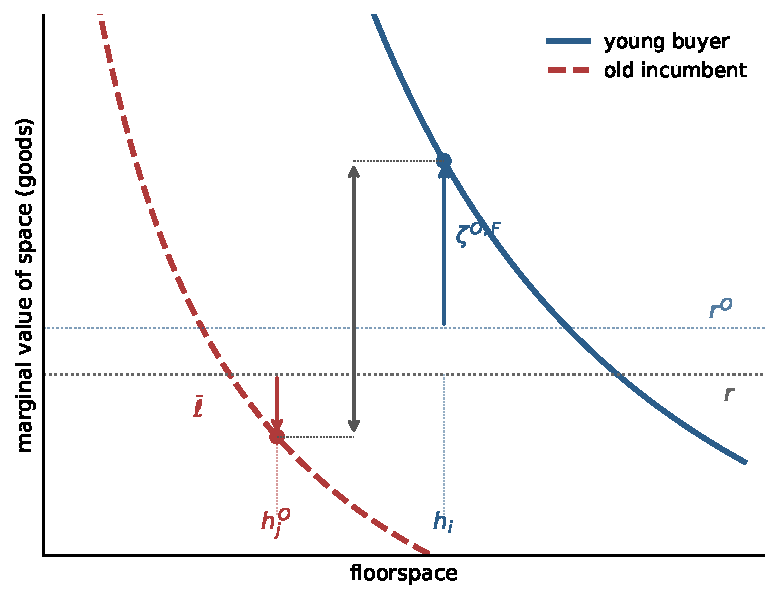
\includegraphics[width=\textwidth,height=0.57\textheight,keepaspectratio]{example_misallocation_only_paper_notation.pdf}
    \column{0.44\textwidth}
      \small
      Moving one unit from a locked-in old incumbent to a financing-constrained young buyer produces surplus
      \[
        \zeta_i^{O,F}+q\bar\ell+\bar\ell>0.
      \]
      \begin{itemize}\setlength{\itemsep}{0.25em}
        \item The buyer values space above effective user cost.
        \item The incumbent values retained space below the market rent because selling realizes a taxable gain.
        \item The common market price cancels.
      \end{itemize}
  \end{columns}
  \source{Circulated note, Proposition 1 and Figure 1.}
\end{frame}

% 9
\begin{frame}{Fertility and Policy}
  \begin{columns}[T,onlytextwidth]
    \column{0.52\textwidth}
      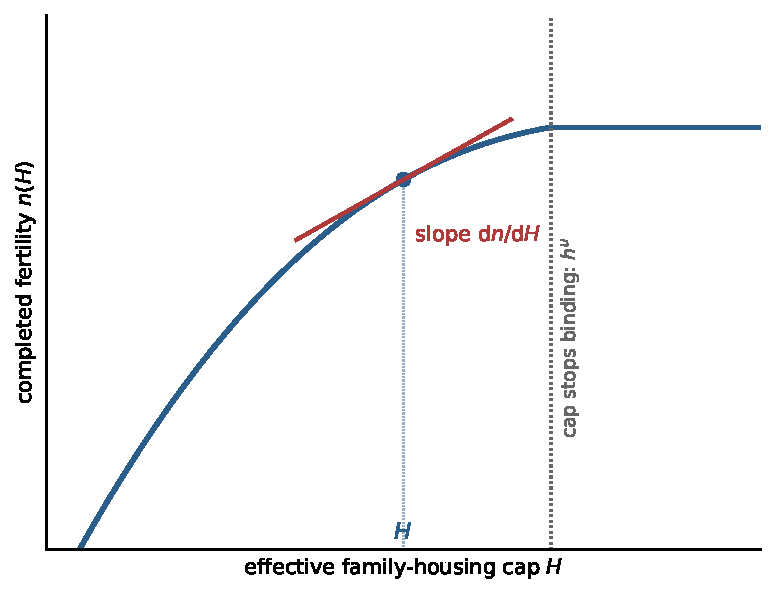
\includegraphics[width=\textwidth,height=0.57\textheight,keepaspectratio]{example_fertility_cap_paper_notation.pdf}
    \column{0.44\textwidth}
      \small
      Along a binding cap, more space has two effects:
      \begin{itemize}\setlength{\itemsep}{0.25em}
        \item it makes the child's housing requirement easier to meet;
        \item it tightens the budget through the cost of additional space.
      \end{itemize}
      Fertility rises when the housing channel dominates:
      \[
        \chi\le (1+\Lambda)\frac{\kappa r^m}{\alpha}.
      \]
      Exposure and pass-through determine the aggregate effect of a housing policy.
  \end{columns}
  \source{Circulated note, Analytical Model: Fertility and policy; Figure 2.}
\end{frame}

% 10
\begin{frame}{Quantitative Lifecycle Model}
  \begin{center}
  \begin{tabular}{c@{\hspace{1.5em}}c@{\hspace{1.5em}}c@{\hspace{1.5em}}c}
    \textbf{18} & \textbf{18--42} & \textbf{66} & \textbf{85}\\
    entry & fertile window & retirement & maximum age
  \end{tabular}
  \end{center}

  \vspace{1em}
  \begin{itemize}\tightitems
    \item Households face persistent earnings risk and save in liquid assets.
    \item A childless household makes a one-time discrete completed-family-size choice; children then age and leave home.
    \item Each period households choose renting or one of five owner sizes and adjust saving.
    \item Entry and the stationary population scale respond in counterfactuals.
  \end{itemize}

  The model preserves the analytical mechanism while adding the lifecycle margins needed for measurement and policy.
  \source{Circulated note, Quantitative Lifecycle Model: Lifecycle and income.}
\end{frame}

% 11
\begin{frame}{Preferences and Bequests}
  Dependent children shift minimum consumption and housing requirements:
  \[
    \bar c(n,s)=\bar c_0+\bar c_n n_s,
    \qquad
    \bar h(n,s)=\bar h_0+\bar h_{\mathrm{jump}}\1\{n_s\ge1\}+\bar h_n n_s.
  \]

  Flow utility is CRRA over residual consumption and usable housing services:
  \[
    u=\frac{\left[(c-\bar c)^{\alpha_c}\mathbf h^{1-\alpha_c}\right]^{1-\sigma}}{1-\sigma}
      +\psi_{\mathrm{child}}n_s,
  \]
  where owners receive service premium $\chi_O$ after household needs are removed.

  At death, households value liquid wealth plus the gross value of the house through a warm-glow bequest motive.
  \source{Circulated note, Quantitative Model: Preferences and bequests.}
\end{frame}

% 12
\begin{frame}{Housing, Tenure, and Budget Constraints}
  \begin{columns}[T,onlytextwidth]
    \column{0.48\textwidth}
      \textbf{Renters}
      \begin{itemize}\tightitems
        \item Choose rooms continuously up to $\bar h^R=6$.
        \item Cannot borrow: $b'\ge0$.
        \item Pay rental user cost $r$.
      \end{itemize}
    \column{0.48\textwidth}
      \textbf{Owners}
      \begin{itemize}\tightitems
        \item Choose $h\in\{2,4,6,8,10\}$ rooms.
        \item Can borrow up to $\phi=0.80$ of house value.
        \item Pay depreciation, property tax, and a 6\% sale cost when adjusting.
      \end{itemize}
  \end{columns}

  \vspace{0.7em}
  Housing supply is upward sloping,
  \[
    H^S(r)=\bar H\left(\frac{r}{\bar r}\right)^\eta,
    \qquad \eta=1.75,
  \]
  so higher demand is absorbed by both quantities and prices.
  \source{Circulated note, Quantitative Model: Housing, finance, and taxes.}
\end{frame}

% 13
\begin{frame}{Family Size, Housing, and Equilibrium}
  A childless household in the fertile window chooses family size first, then its current housing position:
  \[
    n'\in\{0,1,2\},
    \qquad
    h'\in\{0,2,4,6,8,10\}.
  \]

  \begin{itemize}\tightitems
    \item $h'=0$ means renting; positive values are owner rungs.
    \item A positive family-size choice fixes completed fertility and activates dependent-child needs immediately.
    \item Type-I extreme-value shocks smooth both family-size and tenure choices.
    \item The equilibrium combines optimal policies, the stationary distribution, entry and population scale, and housing-market clearing.
  \end{itemize}

  A birth can therefore change tenure and occupied space in the same period, rather than only affecting future housing demand.
  \source{Circulated note, Quantitative Model: Household problem and stationary equilibrium.}
\end{frame}

% 14
\begin{frame}{Calibration}
  \begin{columns}[T,onlytextwidth]
    \column{0.48\textwidth}
      \textbf{Assigned outside estimation}
      \begin{itemize}\tightitems
        \item Lifecycle timing and survival
        \item $\sigma=2$, real return, taxes, depreciation
        \item $\phi=0.80$ and sale cost $6\%$
        \item Income process and housing menus
        \item Supply elasticity and entrant wealth
      \end{itemize}
    \column{0.48\textwidth}
      \textbf{Estimated internally}
      \begin{itemize}\tightitems
        \item Patience and consumption weight
        \item Consumption and housing needs
        \item Value and dispersion of family size
        \item Ownership premium and tenure dispersion
        \item Housing-supply scale and bequests
      \end{itemize}
  \end{columns}

  \vspace{0.5em}
  Fourteen parameters are jointly disciplined by CPS fertility, ACS housing and tenure, and PSID wealth and estate moments.
  \source{Circulated note, Calibration: Tables 1 and 2.}
\end{frame}

% 15
\begin{frame}{Model Fit}
  \centering
  \scriptsize
  \renewcommand{\arraystretch}{0.92}
  \begin{tabularx}{0.98\textwidth}{@{}Yrr@{}}
    \toprule
    Moment & Data & Model \\
    \midrule
    Completed fertility / childlessness & 1.918 / 0.188 & 2.034 / 0.189 \\
    First-child rooms increment & 0.664 & 0.681 \\
    Family ownership gap & 0.168 & 0.219 \\
    Ownership, ages 30--55 & 0.575 & 0.658 \\
    Ownership, ages 25--34 & 0.341 & 0.274 \\
    Ownership, ages 65--75 & 0.764 & 0.954 \\
    Renter rooms / owner--renter rooms gap & 3.805 / 2.419 & 3.963 / 2.323 \\
    Childless-owner share with $\ge6$ rooms & 0.596 & 0.760 \\
    Young liquid wealth / income & 0.179 & 0.328 \\
    Estate median / income & 6.501 & 6.431 \\
    Older nonhousing-wealth share & 0.608 & 0.610 \\
    \bottomrule
  \end{tabularx}

  \vspace{0.45em}
  \normalsize
  The largest tension is excessive persistence in homeownership: young households buy too late, while older households rarely exit ownership.
  \source{Circulated note, Calibration: Target moments and fit.}
\end{frame}

% 16
\begin{frame}{Lifecycle Housing Patterns}
  \centering
  
\includegraphics[width=0.96\textwidth,height=0.68\textheight,keepaspectratio]{quant_lifecycle_equilibrium_repaired_nb120.png}

  \vspace{-0.2em}
  \small
  Homeownership is understated through the mid-thirties and overstated from the early forties onward. The child-at-home profile has the right hump but is delayed and too persistent.
  \source{Circulated note, Lifecycle Housing Patterns, Figure 3.}
\end{frame}

% 17
\begin{frame}{Housing and Family Size at Age 42}
  \centering
  
\includegraphics[width=0.96\textwidth,height=0.68\textheight,keepaspectratio]{quant_decision_rules_repaired_nb120.png}

  \vspace{-0.2em}
  \small
  At age 42, higher-income households choose children and larger homes at lower liquid-wealth levels. The discrete owner ladder generates sharp changes in physical rooms.
  \source{Circulated note, Lifecycle Housing Patterns, Figure 4.}
\end{frame}

% 18
\begin{frame}{Quantitative Evidence on the Mechanism}
  Among fertile renters whose positive-family branch reaches the rental cap:
  \[
    \underbrace{r}_{0.130}
      +
    \underbrace{\zeta_i^R}_{0.178}
      =
    \underbrace{0.307}_{\text{marginal value of another room}}
      =2.37\,r.
  \]

  \begin{center}
  \small
  \begin{tabular}{@{}lrr@{}}
    \toprule
    Holder of owner homes with $\ge6$ rooms & ACS & Model \\
    \midrule
    Households age 46+ & 71.8\% & 80.7\% \\
    Households with no children at home & 54.9\% & 74.8\% \\
    \bottomrule
  \end{tabular}
  \end{center}

  The households facing the highest marginal value of family space are distinct from those holding most of the family-sized owner stock.
  \source{Circulated note, Quantitative Evidence on the Mechanism.}
\end{frame}

% 19
\begin{frame}{Housing Policy}
  \begin{center}
  \renewcommand{\arraystretch}{1.25}
  \begin{tabularx}{0.90\textwidth}{@{}Yrr@{}}
    \toprule
    Policy & $\Delta$ total births & $\Delta$ housing price \\
    \midrule
    Purchase grant for family-sized homes & \textbf{+2.1\%} & +0.90\% \\
    Higher property tax plus purchase grant & \textbf{+2.7\%} & -18.44\% \\
    \bottomrule
  \end{tabularx}
  \end{center}

  \vspace{0.8em}
  \begin{itemize}\tightitems
    \item The grant covers roughly one-third of the required down payment on an eligible home.
    \item The package also raises the annual property-tax rate on owner housing from 1 to 2 percent.
    \item Entry, population, and the housing price adjust in both exercises.
  \end{itemize}
  \source{Circulated note, Housing Policy, Table 5.}
\end{frame}

% 20
\begin{frame}{Conclusion}
  \large
  \begin{itemize}\tightitems
    \item A model of completed fertility with tenure choice, saving, and a lifecycle of housing need.
    \item Children raise housing need; rental limits and down payments make space especially costly for young households.
    \item Older households hold most large owner homes. With retention wedges, a cleared market need not allocate them efficiently.
    \item Aim is policy: purchase assistance raises births, and the tax-plus-grant package changes both access and prices.
  \end{itemize}

  \vspace{0.5em}
  \alert{More work is needed:} sequential fertility, income risk, old-age downsizing, and across-market relocation.
  \source{Circulated note, Conclusion and limitations.}
\end{frame}

\end{document}
